\documentclass[a4paper,12pt]{article}
\usepackage[utf8]{inputenc}
\usepackage{listings}
\usepackage[table]{xcolor}
\usepackage{graphicx}

\graphicspath{{/Users/tom/Documents/Programmieren/ChemBox/Documentation/Images/}}

\usepackage{tikz}
\usetikzlibrary{shapes.geometric, arrows}

\tikzstyle{startstop} = [rectangle, rounded corners, minimum width=3cm, minimum height=1cm,text centered, draw=black, fill=red!30]
\tikzstyle{io} = [trapezium, trapezium left angle=70, trapezium right angle=110, minimum width=3cm, minimum height=1cm, text centered, draw=black, fill=blue!30]
\tikzstyle{process} = [rectangle, minimum width=3cm, minimum height=1cm, text centered, draw=black, fill=orange!30]
\tikzstyle{decision} = [diamond, minimum width=3cm, minimum height=1cm, text centered, draw=black, fill=green!30]
\tikzstyle{arrow} = [thick,->,>=stealth]

\definecolor{codegreen}{rgb}{0,0.6,0}
\definecolor{codegray}{rgb}{0.5,0.5,0.5}
\definecolor{codepurple}{rgb}{0.58,0,0.82}
\definecolor{backcolour}{rgb}{0.95,0.95,0.92}

\lstdefinestyle{mystyle}{
    backgroundcolor=\color{backcolour},   
    commentstyle=\color{codegreen},
    keywordstyle=\color{magenta},
    numberstyle=\tiny\color{codegray},
    stringstyle=\color{codepurple},
    basicstyle=\ttfamily\footnotesize,
    breakatwhitespace=false,         
    breaklines=true,                 
    captionpos=b,                    
    keepspaces=true,                 
    numbers=left,                    
    numbersep=5pt,                  
    showspaces=false,                
    showstringspaces=false,
    showtabs=false,                  
    tabsize=2,
}

\lstset{style=mystyle}


\title{ChemBox Project Documentation}
\author{Tom Schneider}

\begin{document}
\begin{titlepage}
    \begin{center}
        \vspace*{1cm}
        
        \huge ChemBox Project Documentation
        
        \vspace{1cm}
        
        \Large Tom Schneider
        
        \vfill
        
        \textbf{Date:} \today \\
        
        \vspace{1cm}
        
        \textbf{Center Number:} 29065 \\
        \textbf{Candidate Number:} 7638 \\
        
        \vspace{1cm}
        
        \textbf{Ellesmere College}
        
    \end{center}
\end{titlepage}

\tableofcontents

\pagebreak

\section{Analysis}

\subsection{Introduction}

Technology gives us the benefits of saving time and doing work more efficiently. The use of software and technology in chemistry does not only help increase accuracy and decrease human error, but also reduces the time spent performing repetitive tasks by hand. ChemBox is a software project with the aim of creating an interactive, user-friendly and intuitive toolbox for automating and simplifying complex and repetitive tasks that come up on a daily basis for students, educators and professionals in the field of chemistry. The application features a range of different tools that should help chemists work more efficiently and also carry out their work more accurately. ChemBox is split into three distinct modules with different functionalities.\\
\linebreak
The first module is the "ChemCalculator". The aim of this part of the program is to help the user carry out calculations by filling in equations and formulae. Although substituting numbers into predefined equations is a rather trivial task, it leaves a lot of room for human error when it comes to things like converting between units or applying mathematical laws correctly. This module should help the user with the most important and at the same time most trivial tasks in chemistry.\\
\linebreak
The second module, "ChemBalancer", is for balancing chemical equations, as the name already suggests. Chemical equations come up in every lab experiment, calculation or research problem. While balancing short equations made up of very few different elements is arguably a rather easy task, it can get quite tricky when you have to work with a large number of different elements, complex ions or just very long equations. Making just a tiny mistake when balancing an important equation can cause a big set back as it can take long to find small errors like mixing up a 2 with a 3.\\
\linebreak
The third and last module is the "ChemEditor". Visualising molecular structures can play a vital role in understanding a substances chemical properties or understanding interactions with other substances. Drawing molecules out by hand is pretty straight forward. It is knowing when a bond is valid and which atoms bond together and which don't that is the tricky part. Having a tool that can help you make sure the chemical molecule you want to draw can even exist, can be a great help not only for beginner level chemists but also for more experienced chemists.

\newpage

\subsection{Prospective Users}

Chembox will provide valuable tools to a diverse user base, spanning from students to professional chemists. The intuitive and straight forward design will allow users with varying backgrounds and degrees to use ChemBox for their own specific needs.\\
In the early stage, the main users of this system will be pupils and staff attending Ellesmere College, but it could be a goal to make the software available open source to anyone online.\\
Engaging with pupils at the college during the early stages allows for a valuable user feedback loop. This direct interaction with the user group will provide insights into the software's usability, identify potential improvements, and address any specific requirements that may arise within the college context.


\subsection{Specific Objectives}

Through being an A-Level Chemistry student myself, I have learned a lot about using chemical equations and performing calculations as well as balancing chemical equations and visualising chemical substances and molecules. I was able to identify a number calculations that processes that come up on a regular basis and divide them into non-negotiable and nice-to-have objectives.

\subsubsection{Chemical Equations and Calculations - ChemCalculator}

The first module of the program is for performing  calculations which are based on chemical formulae.
Where appropriate the program should allow the user to choose from a range of different units for each calculation, so the user doesn't have to calculate the conversions like the one from $cm^{3}$ to $dm^{3}$ for example.\\
\linebreak
Required functionalities:\\
\linebreak

\begin{enumerate}

\item Standard moles calculation:
\[moles=\frac{mass}{molar\: mass}\]
\item Calculation to find the concentration:
\[concentration=\frac{moles}{volume}\]
\newpage
\item Avogadro's number calculations. The user should be able to give a number of different inputs, including mass, moles, molecular weight and the number of atoms. After giving two independent inputs, the program should be able to calculate the rest of the values using Avogadro's number.\\
The equation the calculator will be based on is:
\[number\: of\: atoms = Avogadro's\: number \times moles\]
This should be paired with a mole calculator for the possibility use the following formula:
\[number\: of\: atoms = Avogadro's\: number \times \frac{mass}{molar\: mass}\]
\item Atom Economy calculation:
\[Atom\: Economy = \frac{Mr\: of\: desired\: product}{Sum\: of\: Mr\: of\: all\: reactants}\times 100\]
\item Percentage Yield calculation:
\[\%Yield = \frac{Actual\: yield}{Theoretical\: yield} \times 100\]
\item Calculation for the Specific Heat Capacity and Enthalpy changes:
\[q = mc {\Delta} T\]
\begin{quote}
(q = energy change) (m = mass) (c = specific heat capacity) (${\Delta}$T = temperature change)
\end{quote}
\item Equilibrium Constant calculation for a reversible reaction:
\[a[A] + b[B] \rightleftharpoons c[C] + d[D]\]
\[K_{C} = \frac{[C]^{c}[D]^{d}}{[A]^{a}[B]^{b}}\]
\begin{quote}
($K_{C}$ = Equilibrium Constant) (Upper case letter = Concentration) (Lower case letter = Moles in Equation)
\end{quote}
\item Rate Equation and Rate constant calculation:
\[Rate = k[A]^{m}[B]^{n}\]

\end{enumerate}

Non-essential objectives:
\begin{enumerate}
\item Gibbs Free Energy calculation:
\[{\Delta}G = {\Delta}H - T{\Delta}S\]
\begin{quote}
(${\Delta}$G = Gibbs Free Energy) (${\Delta}$H = enthalpy)\\
(T = temperature) (${\Delta}$S = entropy)
\end{quote}
\item Acid calculations - pH and $[H^{+}]$
\[pH = -log[H^{+}]\]
\[[H^{+}] = 10^{-pH}\]
\item Acid dissociation constants $K_{a}$ and $pK_{a}$
\[K_{a} = \frac{[H^{+}][A^{-}]}{[HA]}\]
\[pK_{a} = -logK_{a}\]
\[K_{a} = 10^{-pK_{a}}\]
\end{enumerate}

\newpage

\subsubsection{Chemical Equation Balancer - ChemBalancer}

A substantial part of the project will be the ChemBalancer which will be the module that balances chemical equations. This system must be able to take complex unbalanced equations and convert them into a balanced version.\\
It must be able to handle subscript numbers, brackets and complex ions.

\subsubsection{Visualisation of Chemical Molecules - ChemEditor}

The third part of the program will be the ChemEditor module, which can be used for visualising the structures of chemical molecules. This module will require a user-friendly and easy to use interface, with the main focus on the canvas. The user should have the option to choose from a range of different elements what he wants to add to the canvas. In a tool bar, the user should also be able to choose the bond order (single, double, triple) and the charge on each atom. When clicking on an atom, there should be an option to add a bond to another atom or delete the atom.\\
When the user constructs their molecules, ChemEditor will have to conduct real-time checks to ensure that atoms do not exceed their valence electrons and that it is chemically possible to have a molecule with the given structure. \\
The required objectives for this module are:\\

\begin{enumerate}

\item Tool bar:\\
In the tool bar on the top end of the application, there has to be a list of buttons for choosing the element, which must include the most common elements (Carbon, Hydrogen, Sulphur, Chlorine, etc.). There also has to be the option to choose the bond order (single, double or triple bond) as well as choosing the option to form a dative bond. Another essential option in form of buttons should be removing atoms and bonds as well as being able to safe the drawn structures as a document.\\
A possible non-essential enhancement would be getting extra information about atoms upon highlighting as well as getting information like the molar mass and the empirical formula of a molecule after highlighting.
\item Canvas:\\
The canvas is the area in which the user can draw their molecules. There are a number of essential features that must be included here.\\
	\begin{enumerate}
	\item The user must be able to draw atoms by clicking on the canvas.
	\item Upon selecting an existing atom on the canvas, depending on the chosen action type, the user should have different options:
		\begin{enumerate}
		\item When the chosen action type is "Draw", a number of greyed out atoms and bonds to those atoms should be drawn, out of which the user can choose where he wants to place his next atom.
		\item When the chosen action type is "Bond", the program should draw a bond from the selected atom to every existing atom on the canvas, with which a bond would be possible. The colour of those bonds needs to be different to the colour of the actual existing 		bonds, to avoid confusion.
		\end{enumerate}
	\end{enumerate}
\end{enumerate}

\subsection{Current and Proposed Systems}

The current standard is to work out chemical equations or draw molecules on paper. This might make sense for simple equations or small molecules, but it gets less efficient and more difficult as complexity increases. Although there are some software solutions for very specific tasks, there isn't one intuitive and easy to use application that combines the different tasks in one place.\\
\linebreak
Naturally, drawing molecules with pen and paper feels best and is the preferred choice by most people. This project is not here to replace that, it should merely pose as a help for chemists when working certain things out.

\newpage

\section{Documented Design}

\subsection{Introduction to the Documented Design}

In this section, I will outline the decisions, that have outlined the development of the ChemBox project and explain the programming techniques used to implement certain algorithms and structures.\\
The program is written in python, with the aim of using as little external frameworks and dependencies as possible, and therefore creating most of this project from scratch. For the GUI implementation, I chose to use the PyQt6 framework, which is a powerful tool for creating GUI applications in python.\\
\subsection{Code breakdown}

The very first function that is called when running the project is the main() function. The purpose of this function is to create the application (Listing 1: line 2) and apply the styling specified in the $style.css$ file to it. It then creates and displays an instance of the ChemBox class.

\begin{lstlisting}[language=Python, caption=main() function]
def main():
    app = QApplication(sys.argv)

    # Load CSS file
    app.setStyleSheet(open('style.css').read())
    
    main_win = ChemBox()
    main_win.show()
    sys.exit(app.exec())
\end{lstlisting}

\newpage

The ChemBox class is the heart of the program, the point where all the different components are merged together to create one complete application. The class inherits from QMainWindow, which is the standard class from which every PyQt6 application has to inherit, to gain access essential tools for displaying the application. The ChemBox class contains only the constructor, in which the layout of the graphical user interface is specified. The constructor defines the dimensions, the title and geometry of the window. It then creates an instance of the TabBar class, which will act as the central widget of the program. Next, the constructor creates instances of the three big components of the project, ChemCalculator (implemented under parent "SideBar()"), ChemBalancer and ChemEditor, and sets their specific layouts as the layout of their allocated tabs (Listing 2: lines 18 - 25).

\begin{lstlisting}[language=Python, caption=Code snippet of ChemBox class No.1]
class ChemBox(QMainWindow):
    def __init__(self):
        super().__init__()

        # set window properties
        self.__left = 300
        self.__top = 300
        self.__width = 1280
        self.__height = 720
        self.__title = "ChemBox"
        self.setWindowTitle(self.__title)
        self.setGeometry(self.__left, self.__top, self.__width, self.__height)
        self.setFixedSize(self.__width, self.__height)

        self.tab_bar = TabBar()
        self.setCentralWidget(self.tab_bar)

        self.side_bar = SideBar()
        self.tab_bar.tab1.setLayout(self.side_bar.main_layout)

        self.chem_balancer = ChemBalancer()
        self.tab_bar.tab2.setLayout(self.chem_balancer.balancer_layout)

        self.chem_editor = ChemEditor()
        self.tab_bar.tab3.setLayout(self.chem_editor.editor_layout)
\end{lstlisting}

\newpage

This next part of the constructor of the ChemBox class creates instances of every individual component of the ChemCalculator module (Listing 3: lines 1 - 7). After that, each calculator module's layout is set as the corresponding layout for the specified sidebar tabs.

\begin{lstlisting}[language=Python, caption=Code snippet of ChemBox class No.2]
        self.moles_calc = MolesCalculator()
        self.concentration_calc = ConcCalculator()
        self.avogadro_calc = AvogadroCalculator()
        self.ideal_gas_law_calc = IdealGasLawCalculator()
        self.equilibrium_calc = EquilibriumCalculator()
        self.gibbs_calc = GibbsFreeEnergyCalculator()
        self.specific_heat_calc = SpecificHeatCalculator()

        # Initialise moles tab in sidebar
        self.side_bar.moles_tab.setLayout(self.moles_calc.moles_layout)

        # Initialise concentration tab in sidebar
        self.side_bar.conc_tab.setLayout(self.concentration_calc.conc_layout)

        # Initialise avogadro's calculator tab in sidebar
        self.side_bar.avogadro_tab.setLayout(self.avogadro_calc.avogadro_layout)

        # Initialise igl tab in sidebar
        self.side_bar.ideal_gas_tab.setLayout(self.ideal_gas_law_calc.ideal_gas_layout)

        # Initialise equilibrium constant calculator tab
        self.side_bar.equilibrium_tab.setLayout(self.equilibrium_calc.layout)

        # Initialise gibbs free energy calculator
        self.side_bar.gibbs_free_energy_tab.setLayout(self.gibbs_calc.layout)

        # Initialise specific heat energy calculator
        self.side_bar.specific_heat_tab.setLayout(self.specific_heat_calc.layout)
\end{lstlisting}

\newpage

The tab bar is implemented in the $gui\_comps.py$ file, as a simple class, that inherits from QWidget, which allows for the class to have a specific layout. The tab bar is created as a horizontal layout using QHBoxLayout, which means that every widget added to it, lines up horizontally.\\
The QTabWidget holds the widgets, which act as a place holder for the specific layouts of each tab.\\

\begin{lstlisting}[language=Python, caption=TabBar implementation]
from PyQt6.QtWidgets import QTabWidget, QWidget, QHBoxLayout


class TabBar(QWidget):
    def __init__(self):
        super(QWidget, self).__init__()

        self.layout = QHBoxLayout(self)

        self.tabs = QTabWidget()
        self.tab1 = QWidget()
        self.tab2 = QWidget()
        self.tab3 = QWidget()
        self.tabs.addTab(self.tab1, "ChemCalculator")
        self.tabs.addTab(self.tab2, "ChemBalancer")
        self.tabs.addTab(self.tab3, "ChemEditor")

        self.layout.addWidget(self.tabs)
        self.setLayout(self.layout)
\end{lstlisting}


The goal was to achieve a design like the one illustrated in Figure 1, where 1, 2 and 3 in the small boxes at the top of the screen represent buttons in the tab bar.

\begin{figure} [h]
	\centering
	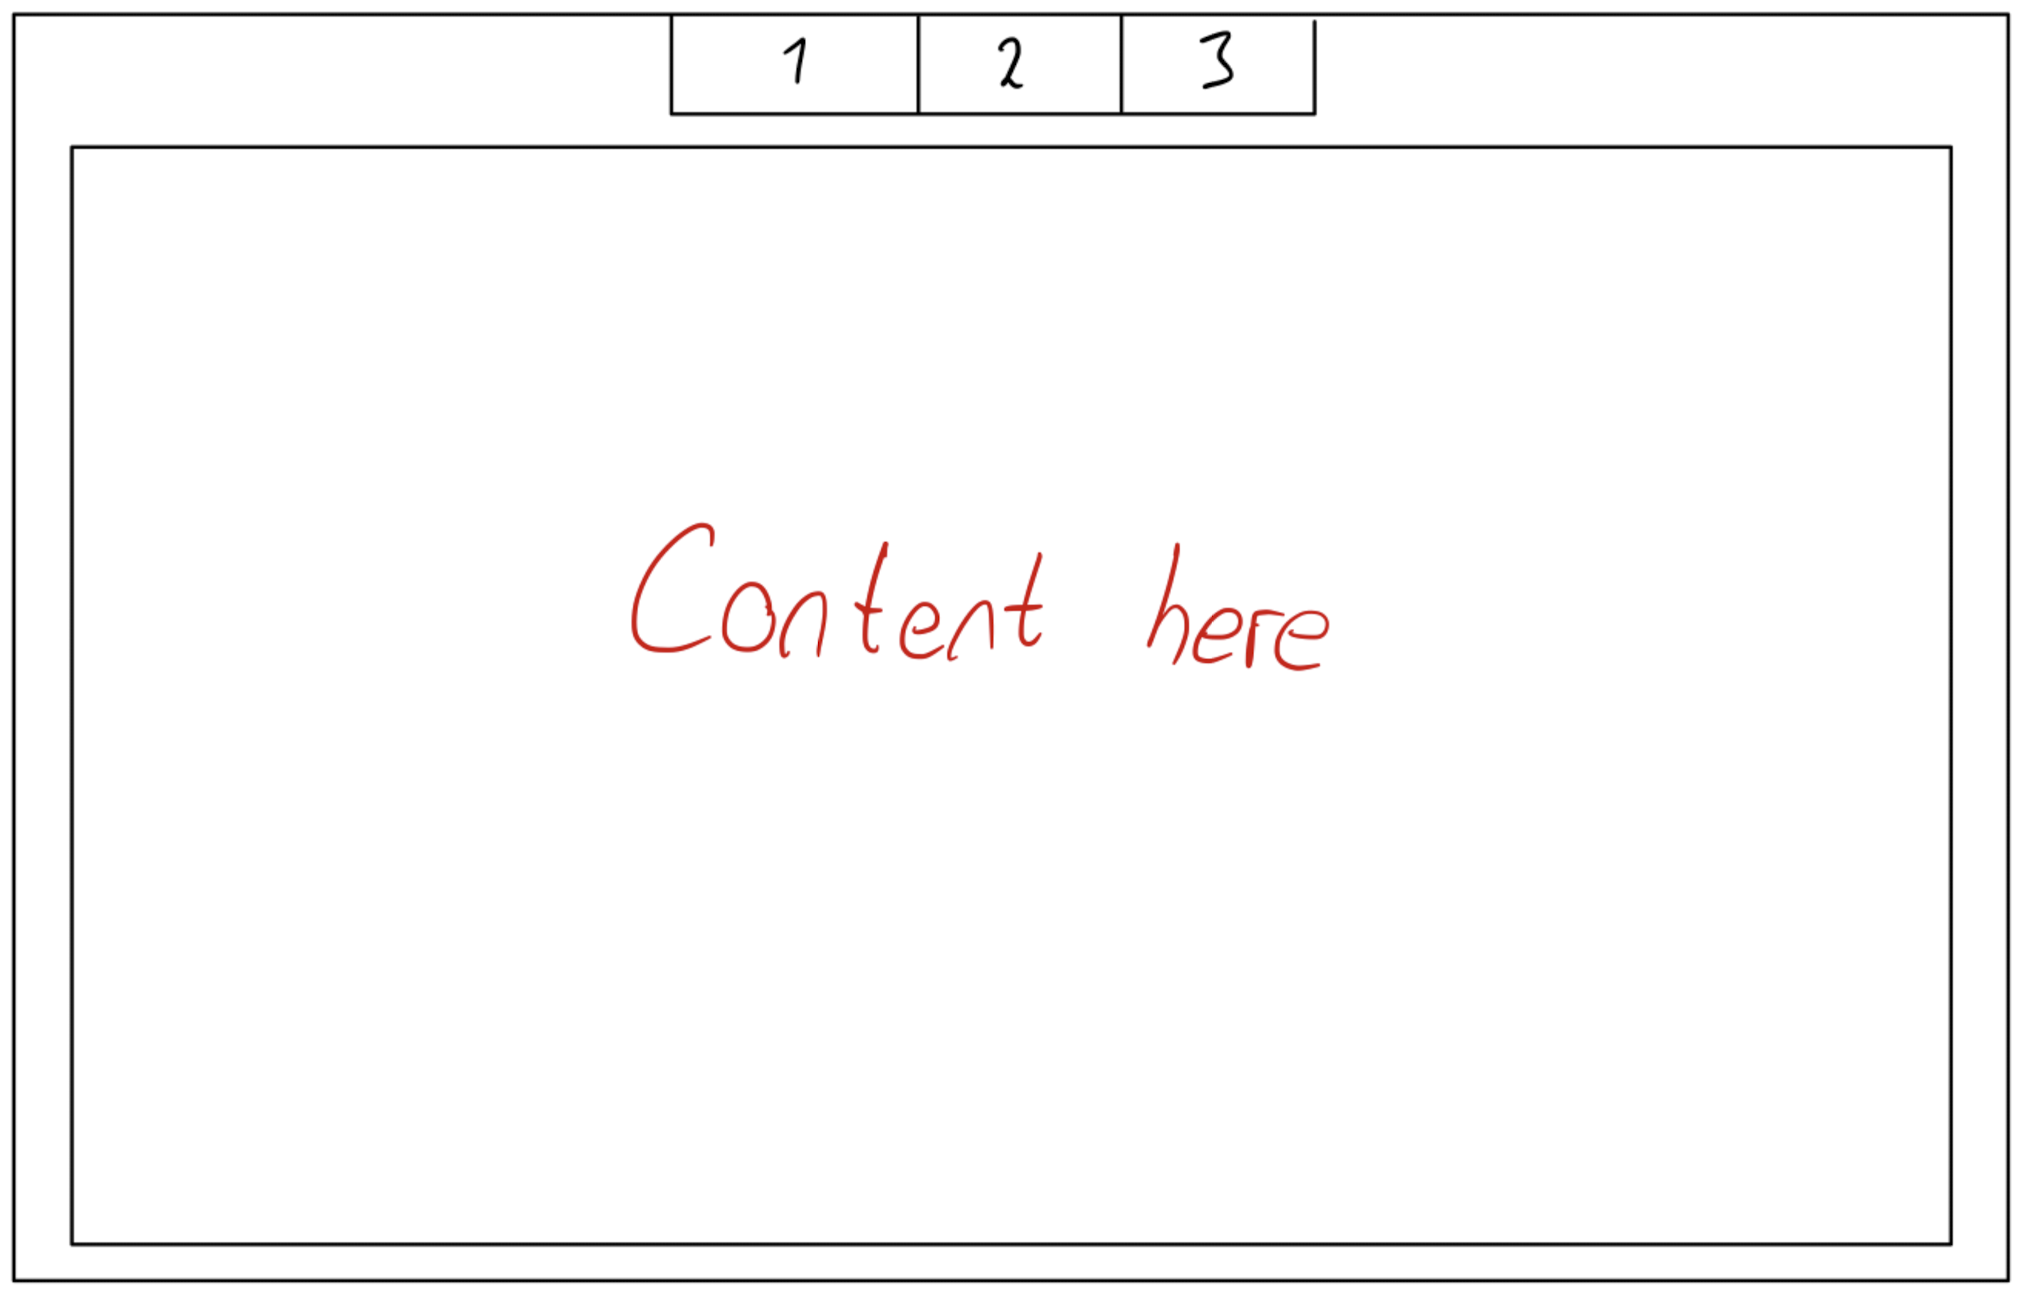
\includegraphics[scale=0.4]{tabs_mockup}
	\caption{Mockup drawing of tab bar}
	\label{fig:tabs_mockup}
\end{figure}
\newpage

When developing the ChemCalculator module, the first issue I encountered was how I would create a layout that would work for multiple separate sub-calculators. I had three different possible systems for displaying the module. The first option was creating a sidebar, where the user a choose the exact calculator they were looking for, and then always displaying the selected one. The second option was very similar, but with an additional tab bar at the top or bottom of the screen. This solution is not very good looking and could cause confusion with the actual tab bar that allows the user to switch between the programs modules. The third option was putting every calculator on the same page, each in it's own area, clearly separated from the others, and make the window scrollable. I decided against this option, as this design could have gotten very messy. Therefore, I decided to create a sidebar for the ChemCalculator. \\
As there is no built-in sidebar widget in PyQt6, I have designed my own way of creating one. I did so by using the QTabWidget, which I also used for the tab bar, but not display it. I was able to benefit from the already existing widget, for the switching between calculators, and use buttons placed on the left side of the screen as a replacement for an actual sidebar. The buttons connect to a method, which changes the the current index of the tab widget to the according number of the calculator, which updates the page that is displayed. This is illustrated in the following code snippet (Listing 5), which only includes the example on a single button, for better readability of this document.

\begin{lstlisting}[language=Python, caption=Sidebar example]
class SideBar(QWidget):
    def __init__(self):
        super(QWidget, self).__init__()
        self.side_bar_layout = QVBoxLayout()
        
        self.gibbs_free_energy_tab_button = QPushButton("Gibbs Free Energy Calculator")

        self.gibbs_free_energy_tab_button.clicked.connect(self.gibbs_free_energy_button)
      
        self.gibbs_free_energy_tab = QWidget()

        # Add buttons to sidebar layout
        self.side_bar_layout.addWidget(self.gibbs_free_energy_tab_button)

        self.side_bar_widget = QWidget()
        self.side_bar_widget.setLayout(self.side_bar_layout)

        self.page_widget = QTabWidget()

        self.page_widget.addTab(self.gibbs_free_energy_tab, "")
        self.page_widget.setCurrentIndex(0)
        self.page_widget.setStyleSheet('''QTabBar::tab{
        width: 0; 
        height: 0; 
        margin: 0; 
        padding: 0; 
        border: none;
        }''')

        self.main_layout = QHBoxLayout()
        self.main_layout.addWidget(self.side_bar_widget)
        self.main_layout.addWidget(self.page_widget)

        self.main_widget = QWidget()
        self.main_widget.setLayout(self.main_layout)
        
    def gibbs_free_energy_button(self):
        self.page_widget.setCurrentIndex(5)
\end{lstlisting}
\newpage

\section{Testing}

\section{Evaluation}
\newpage

\end{document}
